\subsubsection{Deletion}

In deletion, if a data need to be delete, and the bucket is only contain one node or data, then this mapping will be delete, otherwise only the count in the node will minus one. Next, delete the n-gram indexing in all index table.\\

Using the same example in figure \ref{fig:algorithm:string:insertion:example_2}. If removing the $"book"$ which will remove some nodes in both index table, and then the tables should look like figure \ref{fig:algorithm:string:deletion:example_1}. For better understanding, the nodes which need to remove will use the line over it.

\begin{figure}[h]
\centering
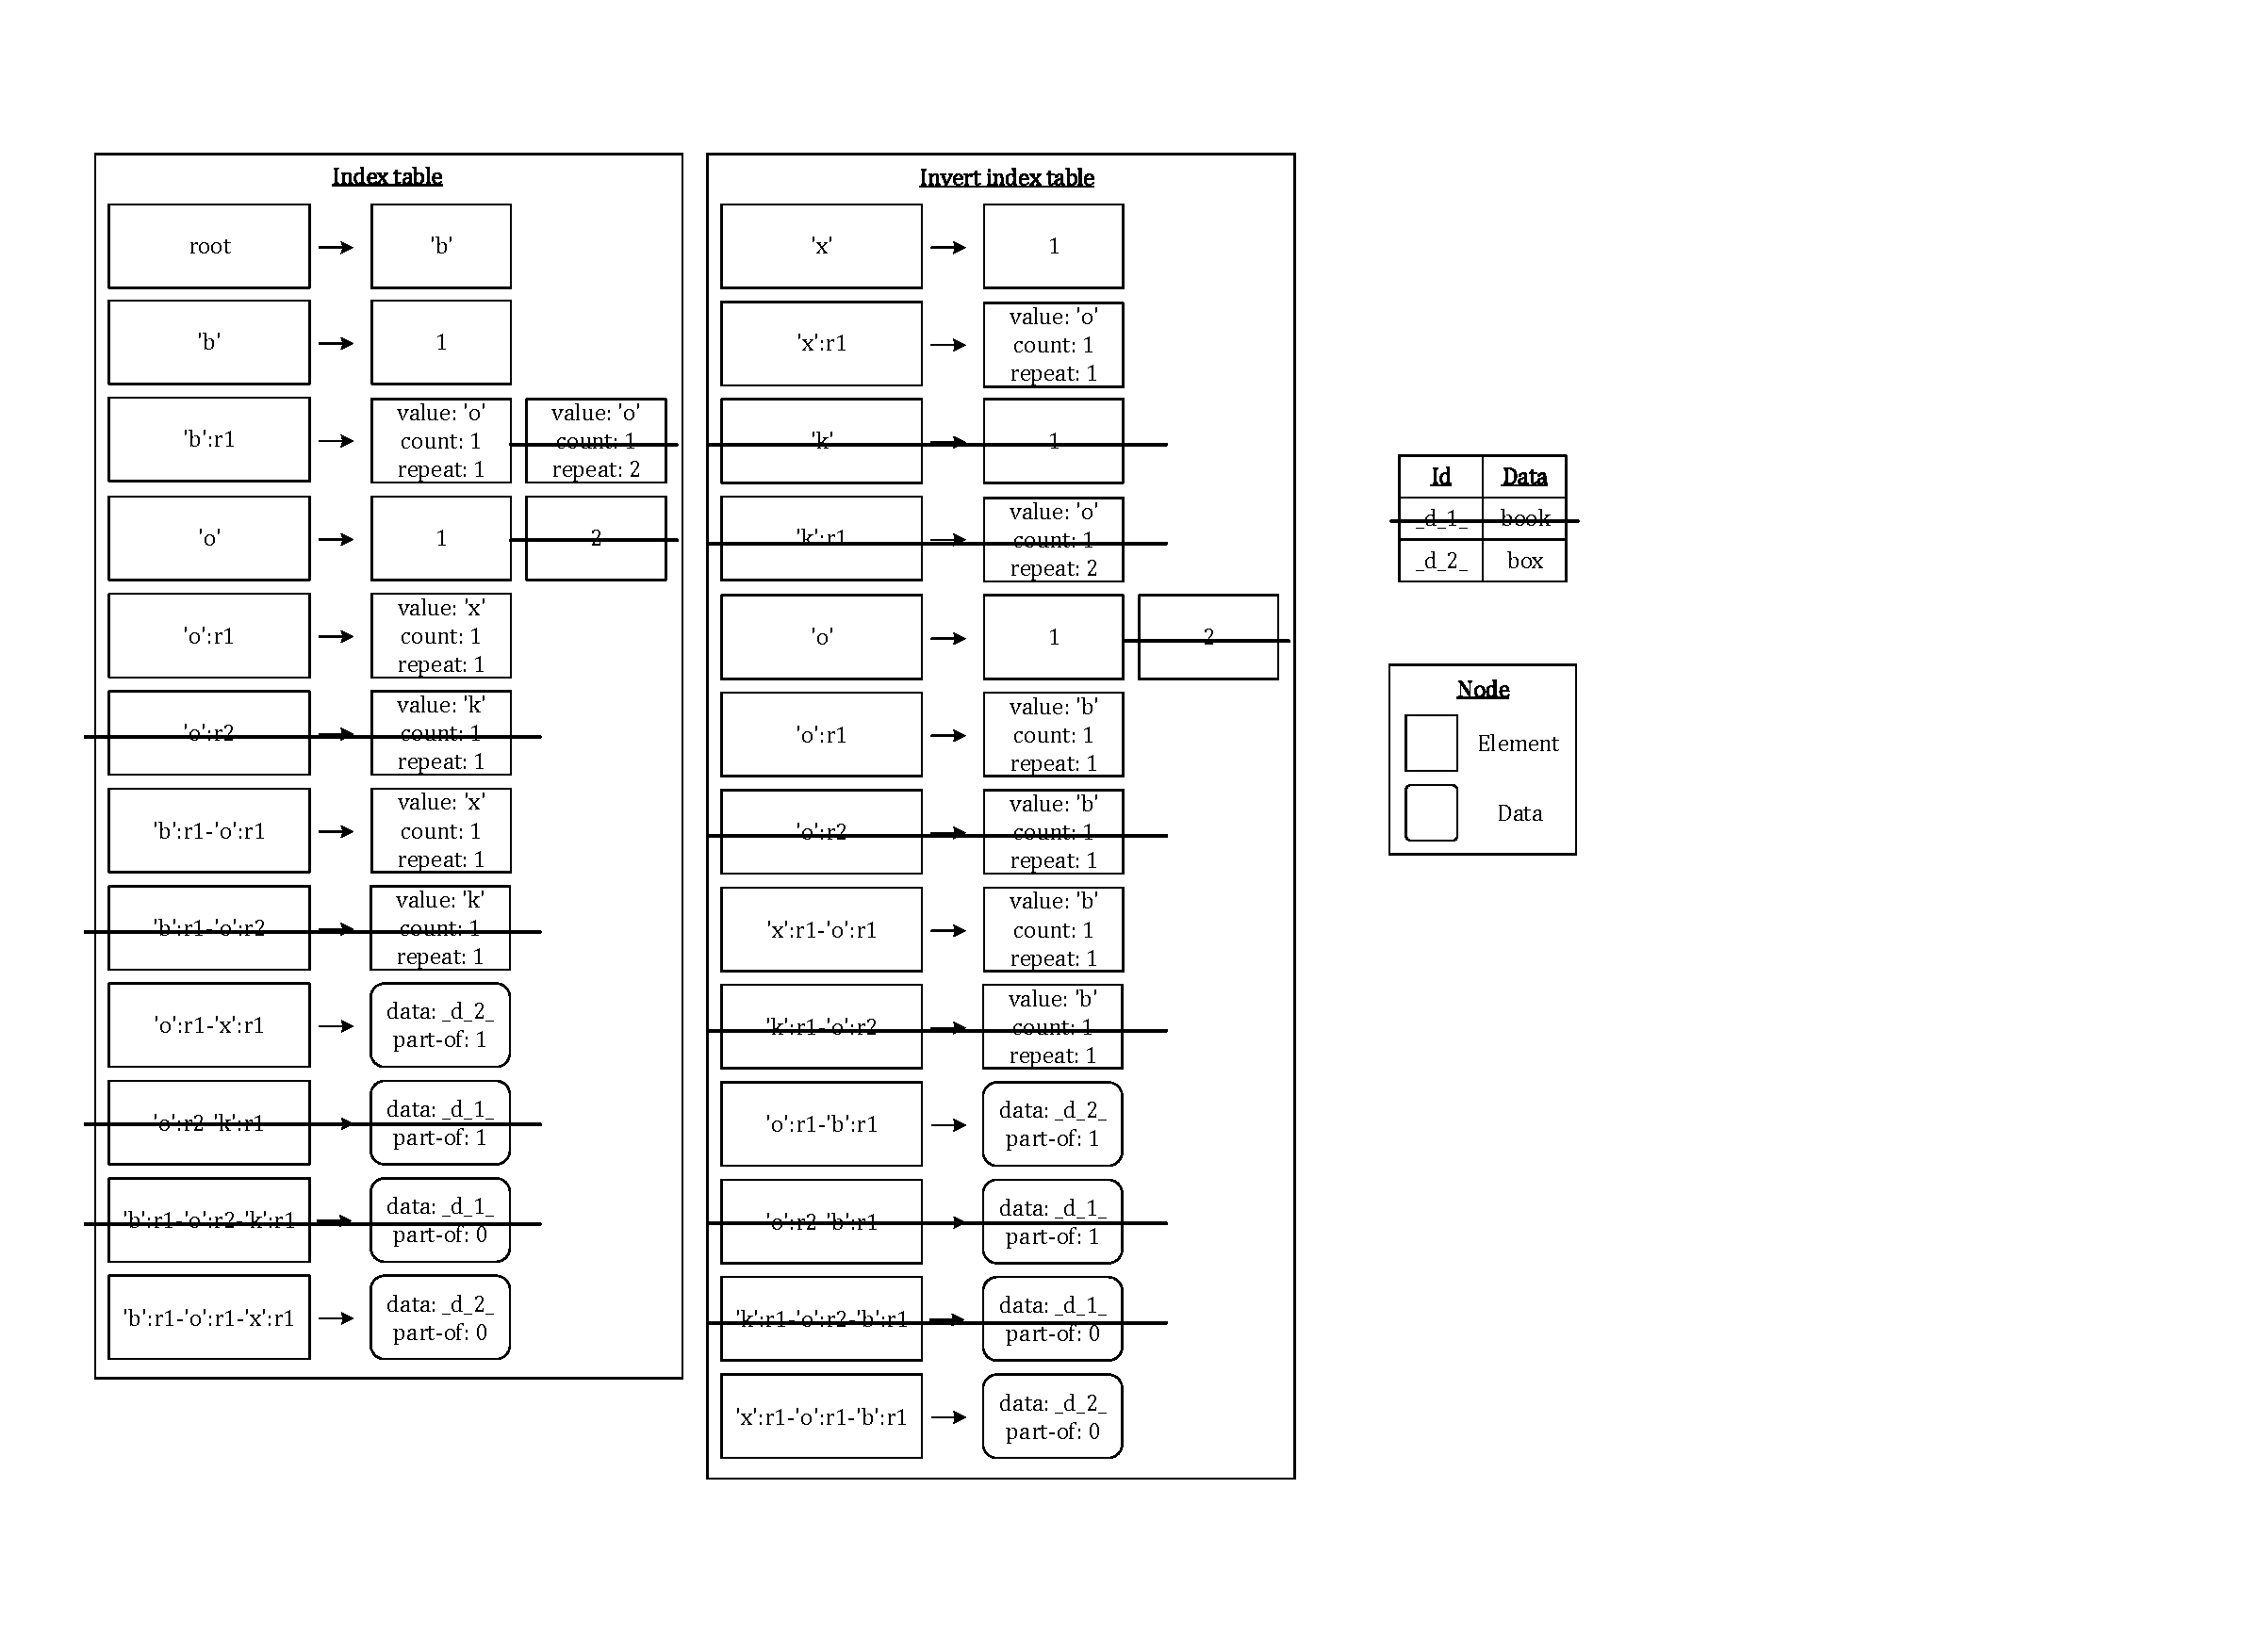
\includegraphics[scale=0.4]{./algorithm/string/pic/deletion/example_1_v3.pdf}
\caption{Delete $"book"$ from table.}
\label{fig:algorithm:string:deletion:example_1}
\end{figure}

The time needed is equals to $2 * O(b!)$, $b$ is the number of for loop which is equal to the byte length of string in one table (Normally it is equal, but in this case $(b = 3)$ which is because the $"o"$ have handled by the repeat counting). Because $2 * O(b!)$ is domain as $O(b)$, so the time complexity of delectation is $O(b)$.

